
%%%%%%%%%%%%%%%%%%%%%%% file typeinst.tex %%%%%%%%%%%%%%%%%%%%%%%%%
%
% This is the LaTeX source for the instructions to authors using
% the LaTeX document class 'llncs.cls' for contributions to
% the Lecture Notes in Computer Sciences series.
% http://www.springer.com/lncs       Springer Heidelberg 2006/05/04
%
% It may be used as a template for your own input - copy it
% to a new file with a new name and use it as the basis
% for your article.
%
% NB: the document class 'llncs' has its own and detailed documentation, see
% ftp://ftp.springer.de/data/pubftp/pub/tex/latex/llncs/latex2e/llncsdoc.pdf
%
%%%%%%%%%%%%%%%%%%%%%%%%%%%%%%%%%%%%%%%%%%%%%%%%%%%%%%%%%%%%%%%%%%%


\documentclass[runningheads,a4paper,10pt]{llncs}

\usepackage{geometry}
\geometry{hmargin=3cm}
\geometry{vmargin=3cm}

% pour les accents utilisés en français 
\usepackage[utf8]{inputenc}
\usepackage[T1]{fontenc}
\usepackage[francais,english]{babel}
\usepackage[hiperref]{}

%\usepackage{amssymb}
\setcounter{tocdepth}{3}

%images config
\usepackage{graphicx}
\graphicspath{ {images/} }

% for matrixes
\usepackage{amsmath}

% for control over itemize
\usepackage{enumitem}

%to put the link to the video
\usepackage{url}
\usepackage[hidelinks]{hyperref}

% for control over itemize
\usepackage{enumitem}

\usepackage[square, authoryear, sectionbib]{natbib} 


\bibliographystyle{apalike}
%\bibliographystyle{splncs03}
%\bibliographystyle{acmsiggraph}



\urldef{\mailsa}\path|samuel.carensac@insa-lyon.fr|    

\begin{document}

\mainmatter  % start of an individual contribution

% first the title is needed
\title{Contrôle du mouvement de marche\\ de personnages virtuels en milieu liquide}

% a short form should be given in case it is too long for the running head
%\titlerunning{Lecture Notes in Computer Science: Authors' Instructions}

% the name(s) of the author(s) follow(s) next
%
% NB: Chinese authors should write their first names(s) in front of
% their surnames. This ensures that the names appear correctly in
% the running heads and the author index.
%
\author{Samuel Carensac}
%
%\authorrunning{Lecture Notes in Computer Science: Authors' Instructions}
% (feature abused for this document to repeat the title also on left hand pages)

% the affiliations are given next; don't give your e-mail address
% unless you accept that it will be published
\institute{Département informatique\\ INSA de LYON \\ 2014/2015\\
\vspace{0.5cm}
\begin{flushleft}
\hspace{1cm}Sous la responsabilité de :\\
\hspace{1cm}nom du tuteur : Saida Bouakaz, Nicolas Pronost\\
\hspace{1cm}nom de l’enseignant : Stéphane Bres
\end{flushleft}
}

%
% NB: a more complex sample for affiliations and the mapping to the
% corresponding authors can be found in the file "llncs.dem"
% (search for the string "\mainmatter" where a contribution starts).
% "llncs.dem" accompanies the document class "llncs.cls".
%

%\toctitle{Lecture Notes in Computer Science}
%\tocauthor{Authors' Instructions}
\maketitle

\selectlanguage{francais}
\begin{abstract}
 L'animation basée physique est de plus en plus étudiée car elle permet de réaliser les interactions avec l'environnement beaucoup plus naturellement. Bien que certains contrôleurs de mouvement permettent la simulation des interactions d'un personnage en milieu liquide ceux-ci ne simulent que la nage. Nous présentons une stratégie de contrôle de mouvement de marche d'un personnage virtuel en immersion partielle dans un liquide. L'effet des liquides sur le mouvement du personnage est modélisé à l'aide de formules d'hydrodynamiques simples. Notre contrôleur permet de combiner différents styles de marches, d'assurer l'équilibre par le placement du pied et d'assurer le contrôle précis de la vitesse du personnage. Nous avons déterminé les paramètres optimaux pour divers critères d'évaluations à l'aide d'une phase d'optimisation. Cette optimisation a été effectuée sur cinq niveaux de liquide régulièrement répartis.
\`A la suite de cette optimisation nous avons conçu un contrôleur capable de s'adapter automatiquement aux variations de niveau d'immersion, de densité du liquide et de vitesses. Notre contrôleur est également robuste à l'application de forces externes.

\keywords{Humain virtuel, Animation basée physique, Contrôle de mouvement, Optimisation hors ligne}
\end{abstract}


\selectlanguage{english}
\begin{abstract}
Physics-based animation is an increasingly studied subject of computer animation because it allows natural interactions with the virtual environment. Though some existing motion controllers can handle the simulation of interactions between a character and a liquid, only few methods focus on the simulation of the locomotion of immersed bipeds. In this paper, we present a control strategy capable of simulating partially immersed gaits. The impact of the liquid on the character's motion is modeled through simple hydrodynamics. To produce natural looking animations, we design a controller allowing the combination of multiple gait styles, the conservation of balance through foot placement and precise control of the character's speed. We determine the optimal parameters for the controller by using an optimization process. This optimization is repeated for several scenarios where the character has to walk across a volume of liquid parametrized by its height. Our controller produces natural looking gaits while being capable of online adaptation to the variation of liquid height, to the modification of the liquid density and to the variation of the required character's speed.
\keywords{ Virtual Human, Physics based animation,  Motion control, Offline optimization }
\end{abstract}



\section{Introduction}

Simulating realistic human motion is a key step in creating virtual environments. Over the years, these environments have become increasingly diverse and complex with a large number of elements that can influence the motion of a virtual character. In those cases, physics-based animation is preferred over kinematic animation since it does not need a series of exact position for each possible interaction. With this increasing complexity, it is difficult to achieve realistic interactions between animated characters and the environment using kinematics-based approaches. Physics-based animation uses physical phenomena (forces and torques) to manipulate the character. This allows the creation of a motion that will be directly impacted by the environment. A growing number of contributions are now working on building controllers using simulated physics~\citep{geijtenbeek2012interactive}. Although they inherently allow obtaining interactions with the environment, the manipulation of the character becomes more complex as no direct control over the position of the limbs of the animated characters is possible.

The main challenge of a controller is to allow high level parametrization of the system. For example, these high level parameters may be the character's speed, the direction of displacement or the motion style. The need to simulate a large number of motion styles (walking, running, jumping...) makes creating a generic controller extremely challenging. Similarly, the mastery of multiple interactions with the environment also increases considerably the complexity of the system. This is why the existing controllers focus on the study of a limited number of motion styles at a time and interactions with the environment~\citep{geijtenbeek2012interactive}. We focused on the control of walking in partial immersion in a liquid. Our objective was to define and implement the necessary mechanisms to a physics-based controller to allow real-time animation of a virtual character interacting with a liquid. Our controller is capable of great freedom of gait style and precise tracking of the character's motion speed.


The remainder of this paper is structured as follows. Section \ref{sec:previous_works} reviews previous works. Then in section ~\ref{sec:overview}, we give an overview of our system. Sections ~\ref{sec:ext_forces} to ~\ref{sec:implementation} describe the tools used in the implemented system. Section~\ref{sec:results} illustrates a variety of results, provides discussions and gives the limits of our method. In section~\ref{sec:conclusion}, we summarize our approach and highlight future areas of work.
 
\section{Previous works}
\label{sec:previous_works}

Numerous works on control of virtual characters with simulated physics can be found in the literature ~\citep{geijtenbeek2012interactive}. Among those works, some share common characteristics with our objectives.

Our work share some features of the SIMBICON (SIMple BIped CONtroler)~\citep{yin2007simbicon} and associated works. Among them, \citep{coros2009robust} propose a system integrating multiple controllers for navigation tasks. The drawback is that the system is designed to use optimization to determine how the different controllers should be used. To enable the use of low gains in the PD-controllers, different methods have been used such as a feedforward system~\citep{yin2007simbicon} or the computation of torques to compensate the effect of gravity~\citep{coros2010generalized}.

\textbf{\textit{Balance control}} is one of the key systems in physics-based simulation. For instance in ~\citep{yin2007simbicon}, secondary PD-controllers are placed on the key joints (stance ankle and swing hip) to dynamically adapt the tracked positions. One way to compute a balance aware foot placement during walk motion is to use an Inverted Pendulum Model (IPM)~\citep{coros2010generalized,kajita20013d}. This model can be used to dynamically compute the trajectory of the swing foot but it limits the range of possible gait styles.

\textbf{\textit{Velocity control}} is often one of the required characteristics of physics-based controllers. Some systems are capable of adapting to online variations of the target velocity. In~\citep{coros2009robust}, multiple controllers are combined for specific motions as forward and backward walks. The IPM based systems offer an inherent control though imprecise as it does not consider the observed velocity~\citep{coros2010generalized}. The use of horizontal virtual forces has been a way to obtain a precise control of the speed and balance of the character~\citep{coros2010generalized,geijtenbeek2012simple}. This system is based on secondary PD-controllers to compute the requisite force. The static gains and constants used in those systems make them unable to track correctly the target velocity when the character is subject to a variable environment (e.g. apparition of a liquid medium). 

\textbf{\textit{Movement in liquids}} have been studied in both simulation~\citep{yang2004layered,si2014realistic} and biomechanics~\citep{barela2006biomechanical,chevutschi2009comparison}. Those works mainly focus either on swimming control or on gait analysis with high level of immersion, making them unusable in our scenarios.
One can also mention~\citep{lentine2011creature} who simulated human walk under wind forces. Most of those works use the Navier-Stockes equations to simulate the liquids making them usually ineffective to obtain real-time and interactive simulations.

To overcome these limitations, we propose a novel controller showing the following characteristics:
\begin{itemize}[noitemsep,nolistsep]
\item{dynamic gait style adaptation by combining multiple reference controllers}
\item{liquid aware gait styles by specific IPM usage and offline optimization}
\item{precise tracking of target velocity by using learning strategies}
\item{real-time interactive simulation by using simple hydrodynamics to simulate the impact of the liquid on the motion}
\end{itemize}

\section{System Overview}
\label{sec:overview}

\begin{figure}[t]
\centering
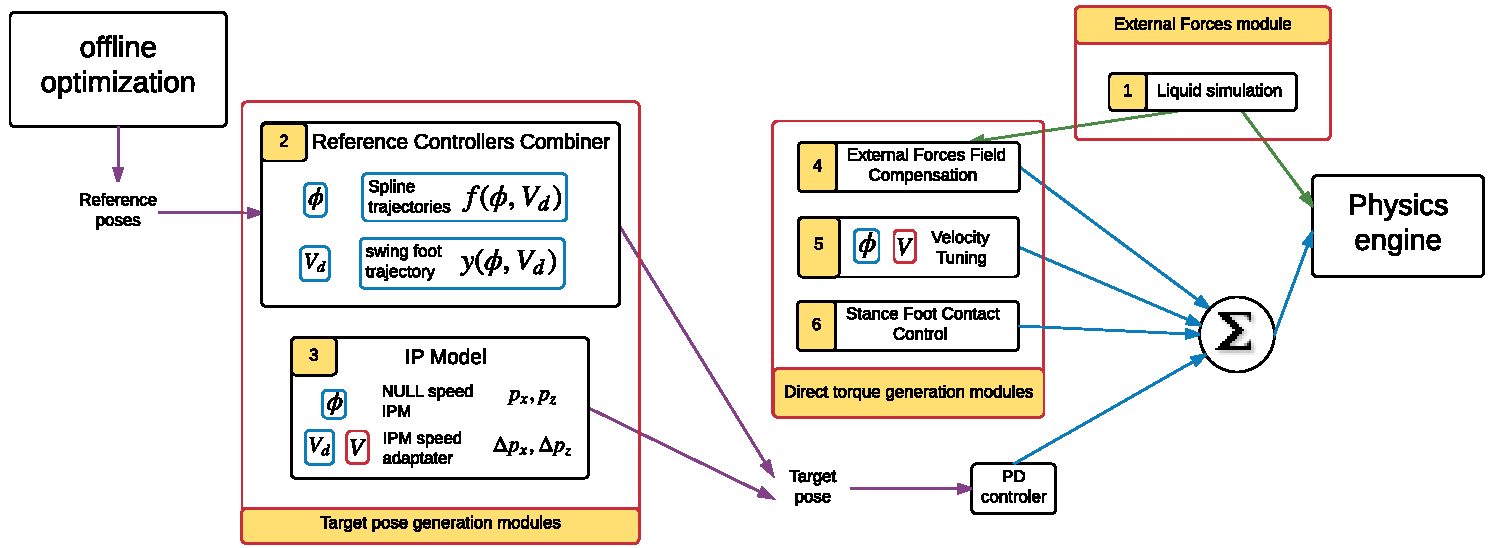
\includegraphics[scale=0.55]{images/general_process.pdf}
\caption{System overview. (1) influence of liquid through external forces; (2) a combination of controllers generating the target poses; (3) an IPM for predictive foot placement; (4) an external force-field compensation helping the PD-controller; (5) velocity tuning for fine corrections of velocity and balance; (6) an active control of the stance foot contact with the ground. $\phi$ is called the phase, and is computed by normalizing the current time $t$ since the last footstrike by the expected step time $T$: $\phi=\frac{t}{T}$.}
\label{fig:shema_controler}
\end{figure}

Our controller consists of six key components that are classified in three categories (figure \ref{fig:shema_controler}). Each one of these categories correspond to one type of interaction with the character: generation of the target pose, generation of torque on the joints and generation of forces applyed on the limbs.

First, we simulate the liquid impact on the character by applying external forces computed by simple hydrodynamics (drag, friction and buoyancy) allowing us to obtain real-time interactions between the liquid and the character (section~\ref{sec:ext_forces}). Our method combines various controllers, each one defining a gait style depending on the simulation conditions (e.g. liquid height, target speed), allowing an adaptive evolution of the gait style (section~\ref{sec:multi_state}). The specified trajectories for the joints composing the swing leg are overridden by the results of an IPM if the character is in the falling phase of a step or if the controller detects a loss of balance (section~\ref{sec:specific_ipm}).

We augment the PD-controller with torques computed through an external force-field compensation. Our system is a extension of Coros et al.'s gravity compensation mechanism~\citep{coros2010generalized} and computes a significant part of the necessary torques (section~\ref{sec:ext_force_comp}).

Our controller includes a precise tracking of the target velocity through an adaptive offset on the swing foot position computed by the IPM (section~\ref{sec:ipm_alt}). Our system presents an improvement of Coros et al.'s fine-scale control~\citep{coros2010generalized} by considering the intra-step speed variation of the character to compute a more efficient virtual force (section~\ref{sec:speed_virt_force}).

We add a feedback controller on the stance ankle that ensure a correct contact between the stance foot and the ground (section~\ref{sec:stance_foot_contact_control}) preventing inadequate movement of the stance ankle in situation not specified in the reference controllers.

Finally, we use offline optimization to generate the reference poses used by the controller combinator. This optimization defines a gait style specific to a given scenario (section~\ref{sec:optimisation}).

\section{External Forces}
\label{sec:ext_forces}

Beside the ground reaction forces, the external forces generated in our system are the forces related to the influence of the liquid on the character. We consider two forces that are based on hydrodynamics laws. The first one is buoyancy. We use the well-known equation $F_{B}=-V_i \rho g$ with $V_i$ the immersed volume of the physics representation of the immersed object and $\rho$ the density of the liquid. The second force is the parasitic drag. We restrict the considered physics phenomena to the form drag and the skin friction, modeling the resulting force $F_D$ using the following equation:
\begin{equation}
F_D=\frac{1}{2} \rho v^2 \times (A_n C_d + S_n C_f)
\end{equation}
where $C_d$ is the drag coefficient, $\rho$ the fluid density, $A_n$ the cross sectional area and $v$ the relative speed to the fluid. Due to the complexity of dynamically computing $C_d$, we set it to 1.0 (average value for a man). $S_n$ is the surface in contact with water for each element and $C_f$ is a coefficient representing the fluid viscosity allowing us a rough representation of the friction. The velocity varying through the limbs, we use a finite elements decomposition of the surface of each limb and compute the parasitic drag for each element individually. The computation of the cross sectional area $A_n$ and the immersion test are both directly realized on each element. We use the same finite elements to obtain an approximation of the surface in contact $S_n$.

\section{Control Framework}
\label{sec:control_framework}

Our system is built on the version of SIMBICON presented in~\citep{coros2010generalized}. The trajectories for the ankles, pelvis, back and head are specified in the coordinate system of the character. This coordinate system is orthonormal, where the z-axis is the sagittal axis of the character, the x-axis is the coronal axis of the character and the y-axis points to the ground. The trajectories for the shoulders, elbows, toes and the knee of the stance leg are specified using local joint coordinates. Unlike~\citep{coros2010generalized}, we allow the user to specify the swing foot trajectory which will give us access to a bigger range of possible motions. 


\subsection{Reference Controllers Combiner}
\label{sec:multi_state}

The goal of the \textit{Controllers Combiner} is to observe dynamic variations of the gait style depending on the conditions of the simulation (e.g. liquid height). Following ~\citep{coros2009robust}, our \textit{Controllers Combiner} is built on multiple reference controllers that are specific to one set of conditions. Even though we limit the conditions to the walking speed and the liquid height, our system could handle other specifications. Each reference controller defines the trajectories for the joints that exhibit significant variations from one standard controller. 
For example, our standard controller is a forward walking controller. It specifies that the heel hits the ground before the toes do. To walk backward, the user has to specify a reference controller stating that the toes hit the ground before the heel and affect a negative sagittal speed to it. Our reference controllers differ from the ones used by ~\citep{coros2009robust} by two characteristics. First, we do not require each individual controller to produce a stable motion. In our system, the balance is acquired by the use of an IPM. 
Second, each individual controller only specifies the joints where the variation from the standard controller is significant. Additionally, our system does not require any optimization step to find the optimal combination of the reference controllers. Instead, when the character ends a step, the system will compute a new trajectory for each joint. Those trajectories are obtained by a square-law interpolation between the two nearest reference controllers. 
For example, given $n$ reference controllers, we will use the two reference trajectories $f_i$ and $f_{i+1}$ defined for the speeds $V_i$ and $V_{i+1}$ to compute the target trajectories $f$: 
$$
f=f_i*(1-R_i)+f_{i+1}*R_i \quad \textrm{with} \quad 0\leq i \leq n
$$
$$
\textrm{and}\quad 
\begin{cases} 
R_i=\left( \frac{V_d-V_i}{V_{i+1}-V_i} \right) ^2   &\textrm{if} \quad   \exists i : V_i < V_d < V_{i+1}\\
R_0=0\\
R_n=1\\
\end{cases}
$$
The same formula is applied to adapt the gait style to the liquid height where the speeds are replaced by heights.

\subsection{Inversed Pendulum Model}
\label{sec:IPM}

We use an \textit{Inversed Pendulum Model} (IPM) supposing constant leg length and zero target velocity similar to the one used in~\citep{coros2010generalized}. We have modified this model to allow the previously impossible specification of some gait styles and to enable a better tracking of the user's target velocity.

\subsubsection{Specific IPM Usage}
\label{sec:specific_ipm}

Our idea to enable the specification of new gait style is that the IPM does not need to control the swing foot during the whole step. We only need to control the position of the swing foot when the character is in a falling state, meaning when the vertical speed of the center of mass is positive $V_{COM}>0$. During a step, the falling phase corresponds to the end of the step. So during the first part of the step we will use a user defined trajectory for the swing foot. This allows the observation of vertical movement of the swing foot without any horizontal movement, which was previously impossible. This kind of gait style is important in our scenarios as it is typical of a character trying to minimize the drag from moving in a liquid.

\subsubsection{IPM Results Alteration}
\label{sec:ipm_alt}

To have a partial control of the velocity, \citep{coros2010generalized} use a linear modification of IPM results depending on the target character velocity ($\Delta(x,z)=-\alpha V_d$). Unfortunately it only works properly near the velocity for which the linear factor has been optimized. In particular, this system cannot handle the transition from an environment with a fluid medium to an unconstrained one.

Our solution is to add a supplementary offset $\Delta(x,z)_i$ to the results of the IPM. This offset will be modified at the end of each step $s$ depending on the difference between the current character velocity and the target velocity $\Delta(x,z)_s = \Delta(x,z)_{s-1}+\beta(V-V_d)$ with $\beta$ a positive constant. The swing foot position from the IP model $P_{IPM}(x,z)$ will therefore be modified as follows:
$$
P(x,z) = P_{IPM}(x,z) - \alpha V_d + \Delta(x,z)_s
$$ 
To prevent parasiting between this system and the velocity tuning (section \ref{sec:speed_virt_force}), we modify the offset only if the virtual force applyed by the velocity tuning reachs $80\%$ of the maximum force allowed. 

\subsection{External Force Fields Compensator}
\label{sec:ext_force_comp}

Our \textit{External Force Fields Compensator} is an extension of the gravity compensation proposed in~\citep{coros2010generalized}. The goal is to dynamically compute a part of the necessary torques at each joint thus permitting the use of lower gains in the main PD-controller. Using virtual forces opposing the external force fields affecting the character gives us a good estimation of these torques. The external forces that we consider are the weight $P=mg$ of each body part of the character and buoyancy $F_B=-\rho V_i$.
To prevent time consuming computation resulting from the application of numerous small virtual forces (depending on the precision of the finite elements), we chose to ignore the liquid drag in the compensator.
 So the final virtual force applied to each body part is:
$$
F=-mg+\rho V_i
$$



\subsection{Velocity Tuning}
\label{sec:speed_virt_force}




In~\citep{coros2010generalized}, the controller applies a horizontal virtual force to the center of mass to obtain a fine control of the speed and balance. Our version presents three major differences. 


\textit{Articuled chain}. Instead of considering one chain that goes from the head to the stance foot our system preconises two chains: the first goes from the pelvis to the stance foot and the second only contains the joint between the pelvis and the torso.
This modification comes from the following two considerations. First, we do not consider the head in the top chain because we do not want the character to tilt the head to control its velocity. Secondly, we separate the torso from the lower body to prevent the character from applying a large torque on the ankle when tilting the torso is enough. 

\textit{Limbs mass impact}. Applying small torques on joints that control the heavier limbs gives a more natural motion than applying important torques to minor joints. Considering this rule we have modified our Jacobian matrix so it takes into account the mass $M_i$ of each individual limb:
$$
J_n ^T (p)=\frac{1}{M}\sum_{\substack{0<i\leq n}} ((P_i(x,y,z)-P_{i-1}(x,y,z))*M_i)
$$
where $M$ is the sum of the limbs' mass considered in the velocity tuning, $P_i(x,y,z)$ the position of the $i$ joint and $P_0(x,y,z)$ the application point of the virtual force. 

\begin{figure*}[t]
\centering
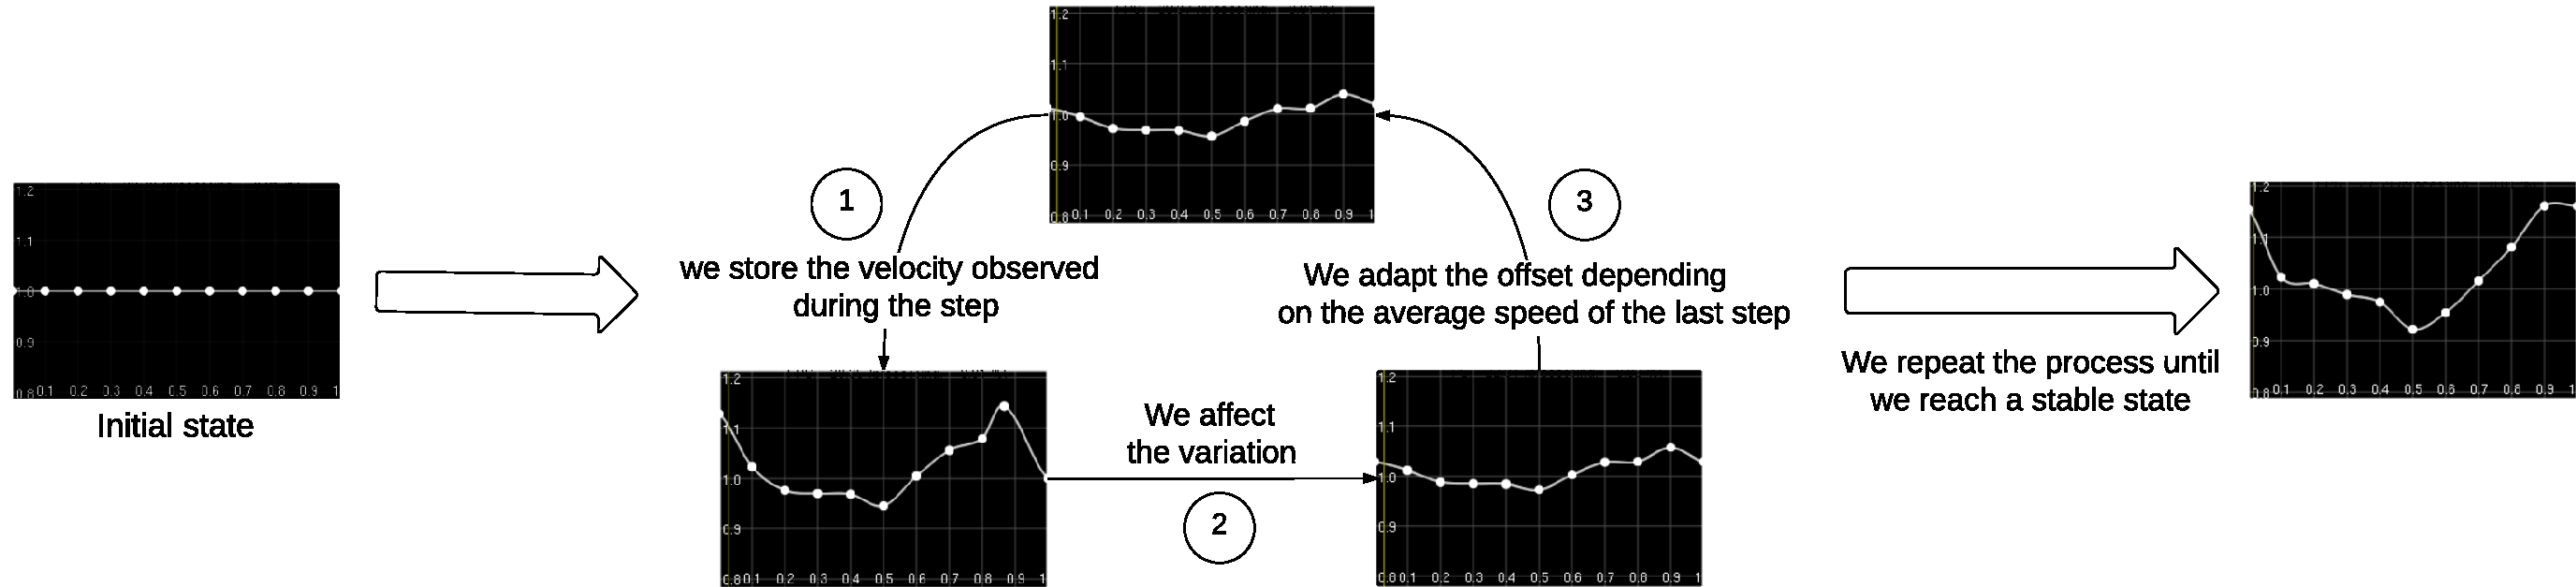
\includegraphics[scale=0.3]{images/speed_curve_learner.pdf}
\caption{Process of learning the required velocity curve}
\label{fig:speed_curve_learner}
\end{figure*}

\textit{Intra-step velocity variations}. In most cases, the velocity is not constant during a step. In most gait styles the character is faster at the start and end of a step than near the middle of it. Supposing it constant as in~\citep{coros2010generalized} may cause the apparition of undesired behaviors where the controller requests the character to slow down at the start of the step, then speed up near the middle of it, and to slow down once again at heel strike. To limit this issue, we use a system to learn the target velocity at each instant of a step that is needed to produce a virtual force as constant as possible. This constant virtual force would result in the character moving at the global target velocity. The \textit{learning velocity curve} is defined by $k$ key points uniformly distributed. The values between those points are computed using Catmull-Rom splines. Our tests have shown that a value of $k=11$ gives enough precision without being too time consuming.
The learning method is based on an iterative principle (see figure~\ref{fig:speed_curve_learner}). During a step we record the velocity of the center of mass of the character. When the step ends, we check if the average variation $\Delta_{avg}$ between the learning velocity curve and the velocity curve observed during the step $f_{obs}$ is lower than a threshold. If so, we move each reference point of the learning velocity curve towards the values read in the observed velocity curve. To help converging without oscillations, we limit the maximum variation that can be affected to each key point to the average variation $\Delta_{avg}$. 

To control the velocity of the character we maintain an offset $K_{off}$ for each curve that will be added when reading the values. At the end of each step we add the observed error $Err = V_d - V_{obs}$ to the offset. To accelerate the convergence to a stable state, we added some rules that limit the evolution of the offset depending on how the velocity trajectory has evolved. The most notable rule is to lower the $Err$ by half of the average variation affected to the curve. So, at the end of the step $s$, each key point $f_s(i)$ is computed with the following equation:

\begin{equation}
\begin{cases}
f_s(i)= (f_{s-1}(i) + min(\Delta_{avg},f_{obs}(i) - f_{s-1}(i))) \\ 
K_{off}(s)=K_{off}(s-1)+  (V_d - V_{obs})*K_{evo\_speed}
\end{cases}
\end{equation}

With $K_{evo\_speed}$ a coefficient set to $1.0$ for the sagittal axis and to $0.2$ for the coronal axis.
If the average variation $\Delta_{avg}$ is above the threshold it means the character is not in a stable motion anymore.
In that case, we stop adapting our learning curve and switch to the use of recovery steps. This means the controller will then ignore the user specified swing foot trajectory and use the trajectory defined by the IPM for the totality of the step. The controller stays in recovery mode until the average variation between the observed speed and the specified one is lower than the threshold. If it takes more than five steps we reset the learning curve to the constant target value and we start learning again. 

\subsection{Stance Foot Contact Control}
\label{sec:stance_foot_contact_control}

When the character loses its balance or when conditions of the simulation deviate from the ones for the references controllers (coronal velocity, liquids with different characteristics…) the specified trajectories may become inadequate. This problem is most apparent on the stance ankle. An inadequate trajectory will lead to a bad contact between the foot and the ground. If the foot is not anchored correctly on the ground a rotation on the stance hip will lead to a rotation of the stance leg instead of the desired rotation of the pelvis. To prevent those situations we add a supplementary torque $\tau _{contact}$ on the stance ankle that ensures a correct contact with the ground. We consider that the contact is correct if the sum of the vertical component of the ground reaction forces applied on the left side and right side of the foot stays higher than $10\%$ of the sum of all the ground reaction forces on the stance foot. We use the same rule to ensure the balance between the front and the back. If needed the torque $\tau _{contact}$ is computed with the following equations:
\begin{equation}
\begin{cases}
\tau _{contact}(x)= (0.1- R_{F/B}) * K_{sag}\\
\tau _{contact}(z)= (0.1- R_{L/R}) * K_{cor}
\end{cases}
\end{equation}
With $R_{F/B}$ (resp. $R_{L/R}$) being the ratio of either front or back forces (resp. left or right) that is under the $10\%$ limit. $K_{sag}$ and $K_{cor}$ are gains similar to the ones used in the PD-controlers. Our experiments have shown that a value of 300 for both of them gives correct results.

\section{Offline Optimization}
\label{sec:optimisation}

The goal of the offline optimization is to find the optimal parameters of our controller for a given scenario (target character's sagittal speed and liquid height). The considered parameters are the 51 key points for the trajectory of the following elements: pelvis, joint between the pelvis and the torso (first Lumbar vertebrae), stance ankle, swing ankle, stance knee, swing foot.

\subsection{Objective function}
During our optimization we use the following evaluation function:
\begin{equation}
f_{eval} =\sum_{\substack{t<k}} (\eta f_{energ} + \beta f_{drag} + \gamma f_{acc}) *(1+0.1* R_{ipm\_alt}) 
+ f_{speed} + f_{balance} + f_{phase}
\label{eq:complete_eval}
\end{equation}
where $k$ is the duration in seconds of the evaluation. This function can be separated in two parts. The first part corresponds to the sum and defines the characteristics of the motion that we want to observe once the optimization is complete. We use a weighted sum of three functions, each one defining a specific behavior:
\begin{itemize}
\item{\textit{Minimization of consumed energy} ($f_{energ}$). The goal of this function is to obtain a motion using the minimum energy possible. This property is measured by the sum of norm of the torques at every joint: $f_{energ}=\sum_{\substack{i}}{|| \tau_i ||}$} 
\item{\textit{Minimization of the drag}. ($f_{drag}$). Using this function, the character tries to move out of the liquid and we prevent velocity spikes within the liquid. We evaluate this property by using the sum of the torques induced by the drag forces on the parent joint of the limb where the drag forces $F_j$ are applied: $f_{energ}=\sum_{\substack{i}}\sum_{\substack{j}}((P_j(x,y,z)-P_i(x,y,z)) \times F_j)$ with  $P_j(x,y,z)$ the force application point and $P_i(x,y,z)$ the position of the parent joint.}
\item{\textit{Minimization of angular acceleration} ($f_{acc}$). The goal of this function is to obtain smooth motions. We estimate the smoothness from the sum of the square of the angular accelerations weigthed by the mass of the corresponding limb in the reference poses $\ddot{\theta_d}_i$ and in the resulting motion $\ddot{\theta}_i$. We use two coefficients to favor minimizing the accelerations of the actual motion: $f_{acc}=\sum_{\substack{i}}M_i*(0.25*\ddot{\theta_d}_i^2+0.75*\ddot{\theta}_i^2)$ }
\end{itemize}

The second part of the evaluation function consists of functions limiting the search space:
\begin{itemize}
\item{\textit{Penalization of IPM alteration} ($R_{ipm\_alt}$). The IPM alteration system is of great influence on the resulting motion. Even with reference poses defined to walk backward our system could succeed in walking forward if asked. To prevent this kind of situations, we penalize simulations heavily relying on the IPM alterations. To do so, we use the ratio between the IPM alteration required to obtain a stable motion ($\Delta(x,z)$) and its maximum threshold $max(\Delta(x,z))$ (0.09 in our tests): $R_{ipm\_alt}=\frac{\Delta(x,z)}{max(\Delta(x,z))}$}
\item{\textit{Velocity tracking} ($f_{speed}$). The goal of this function is to eliminate the simulations where the convergence to the target velocity takes too long (possibly due to unsuitable reference trajectories). We use a high penalization value if the error on the velocity tracking is superior to 1\% of the target velocity: if $||V-V_d||>0.01*||V_d||$ then $f_{speed}=10^{10}$}
\item{\textit{Motion balance} ($f_{balance}$). With this function, we verify if we have a stable motion by refusing simulations using recovery steps. If the system uses at least one recovery step, a high penalization value is given: $f_{balance}=10^{15}$}
\item{\textit{Phase limits} ($f_{phase}$). This function is here to prevent generating motions that could easily reach a phase $\phi$ of 1.0 or that end steps at really low phases which limit our control on the character. In those cases, a high penalization value is given: if $\phi>0.95$ or $\phi<0.7$ at the end of a step then $f_{phase}=10^{10}$}
\end{itemize}

\subsection{Optimization strategy}
Our fitness landscape presents many local minimums. As several physics-based animation systems~\citep{geijtenbeek2012simple,tan2011articulated}, we use a Covariance Matrix Adaptation (CMA)~\citep{hansen2006cma} to explore it.


\section{Implementation}
\label{sec:implementation}
The physics engine used is Open Dynamics Engine (ODE). The simulation step size is $5 \times 10^{-4}s$. The human model used is composed of 28 degrees of freedom, see \citep{coros2009robust} for more details. Collisions between the character's limbs are not considered. The gains of the PD-controller are kept constant through the simulation, and are the same as in the forward walking controller of~\citep{coros2009robust}. Joint torques are limited to $|\tau|<200Nm$  for the hips and knees and $|\tau|<100Nm$  for the other joints. The simulations are performed with a single-thread implementation on a common laptop with 8GB RAM and a 2.5GHz i5 processor. The controller proposed in this section as been build using a liquid with characteristics similar to water: $\rho=1000kg.m^{-3}$ and $\mu=1$. To compute the drag on any body part, we use finite elements around $0.02cm \times 0.02cm$.


\section{Results}
\label{sec:results}

All the results are best seen in the accompanying video. (\href{https://drive.google.com/folderview?id=0B6n5UVMEGbGHfjM5a1phUHZGaUtLNVRNanFDT2xRd19zN0x1UmNabjlCVGN6c1ZFdWRLczA&usp=sharing}{link to the video}).
%%% mettre lien vers la video %%%

\subsection{Offline Optimization}
We report here the impact of the three main criteria in the evaluation function:
\begin{itemize}
\item\begin{minipage}[t]{\linewidth}{
The \textit{minimization of consumed energy} leads to steps keeping the swing foot near the ground in absence of water. When partially immersed, the character keeps the swing foot low but elevates it a bit higher to align the foot with the direction of the foot's velocity.}
\end{minipage}
\item\begin{minipage}[t]{\linewidth}{
The \textit{minimization of the liquid drag} leads to motions keeping the foot outside the water as long as possible until the water height is too high to do so (the limit is a bit above 0.5m which correspond to the knee height). It is interesting to note that the character uses a lateral movement to get the foot out of the water as fast as possible but it does not strike as natural looking.}
\end{minipage}
\item\begin{minipage}[t]{\linewidth}{
The \textit{minimization of angular accelerations} leads to smooth motions keeping the swing foot near the ground with any water height but which prevents the character to recover from external pushes.}
\end{minipage}
\end{itemize}
We experimented on the weights of the evaluation function, among which the two configurations ($\eta=2$, $\beta=8$, $\gamma=1$) and (4,5,1). The first one of the two provoked the apparition of unnatural lateral displacements of the swing foot similar to our observations of the $f_{drag}$ criteria. The second leaded to movements that would choose to stay underwater even for quite low water heights (under the knee). Finally, we have chosen to use the weights (3,6,1) to build our final controller. This combination leads to motions significantly influenced by the water height while keeping a natural looking movement. With these weights, we have created 10 reference controllers. We have two sets of reference controllers corresponding to the character's speeds $0.3m.s^{-1}$ and $0.7m.s^{-1}$. Each set contains one controller for each of the five following water heights: 0, 0.25, 0.5, 0.75 and 1 meter. Each optimization step has been realized with the following stages: 10 gait steps to stabilize the motion, then five seconds for the evaluation. The optimization of a set of five liquid heights for one speed took around 9 hours.

\subsection{Experiments on the final controller}
\begin{figure}[t]
\centering
\begin{minipage}{0.4\columnwidth}
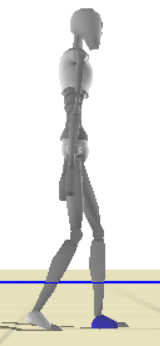
\includegraphics[width=0.101\columnwidth]{images/strips/0_25/1.png}
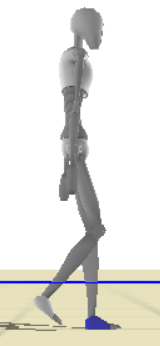
\includegraphics[width=0.101\columnwidth]{images/strips/0_25/2.png}
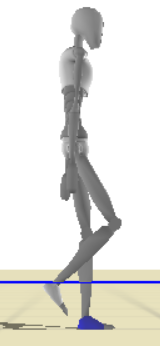
\includegraphics[width=0.101\columnwidth]{images/strips/0_25/3.png}
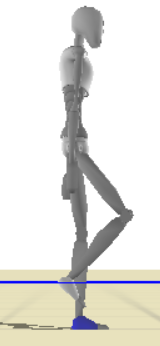
\includegraphics[width=0.101\columnwidth]{images/strips/0_25/4.png}
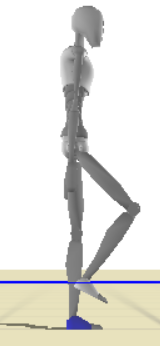
\includegraphics[width=0.101\columnwidth]{images/strips/0_25/5.png}
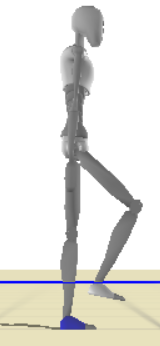
\includegraphics[width=0.101\columnwidth]{images/strips/0_25/6.png}
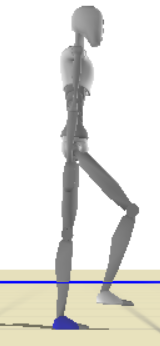
\includegraphics[width=0.101\columnwidth]{images/strips/0_25/7.png}
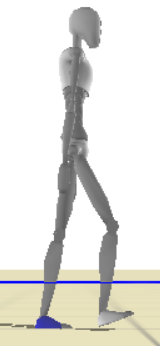
\includegraphics[width=0.101\columnwidth]{images/strips/0_25/8.png}

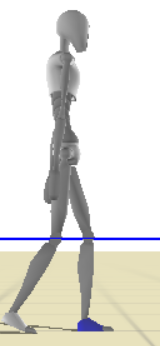
\includegraphics[width=0.101\columnwidth]{images/strips/0_5/1.png}
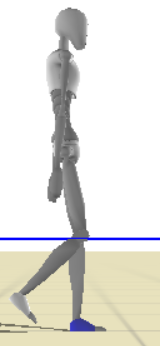
\includegraphics[width=0.101\columnwidth]{images/strips/0_5/2.png}
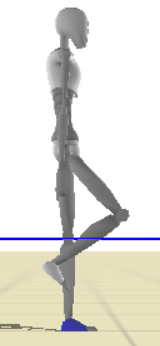
\includegraphics[width=0.101\columnwidth]{images/strips/0_5/3.png}
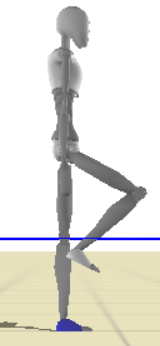
\includegraphics[width=0.101\columnwidth]{images/strips/0_5/4.png}
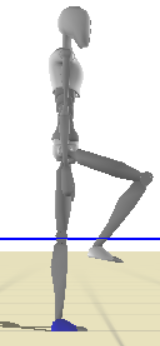
\includegraphics[width=0.101\columnwidth]{images/strips/0_5/5.png}
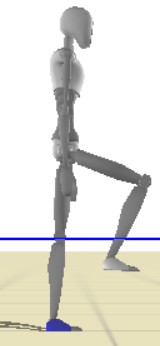
\includegraphics[width=0.101\columnwidth]{images/strips/0_5/6.png}
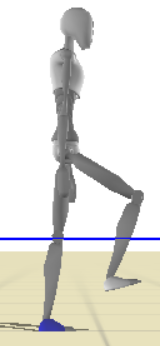
\includegraphics[width=0.101\columnwidth]{images/strips/0_5/7.png}
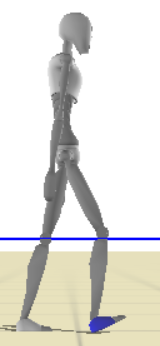
\includegraphics[width=0.101\columnwidth]{images/strips/0_5/8.png}

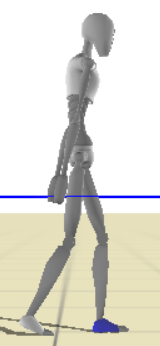
\includegraphics[width=0.101\columnwidth]{images/strips/0_75/1.png}
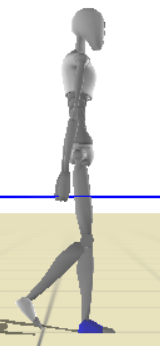
\includegraphics[width=0.101\columnwidth]{images/strips/0_75/2.png}
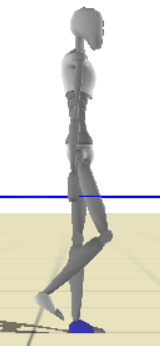
\includegraphics[width=0.101\columnwidth]{images/strips/0_75/3.png}
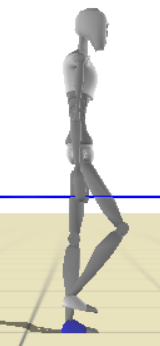
\includegraphics[width=0.101\columnwidth]{images/strips/0_75/4.png}
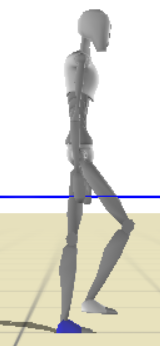
\includegraphics[width=0.101\columnwidth]{images/strips/0_75/5.png}
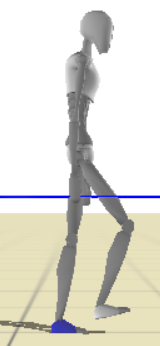
\includegraphics[width=0.101\columnwidth]{images/strips/0_75/6.png}
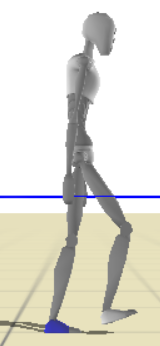
\includegraphics[width=0.101\columnwidth]{images/strips/0_75/7.png}
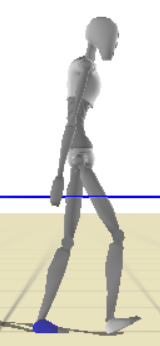
\includegraphics[width=0.101\columnwidth]{images/strips/0_75/8.png}
\end{minipage}
\begin{minipage}{0.55\columnwidth}
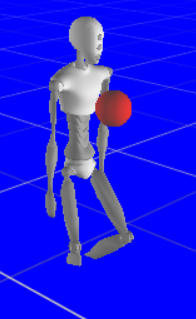
\includegraphics[scale=0.28]{images/strips/ball/img_impact.png}
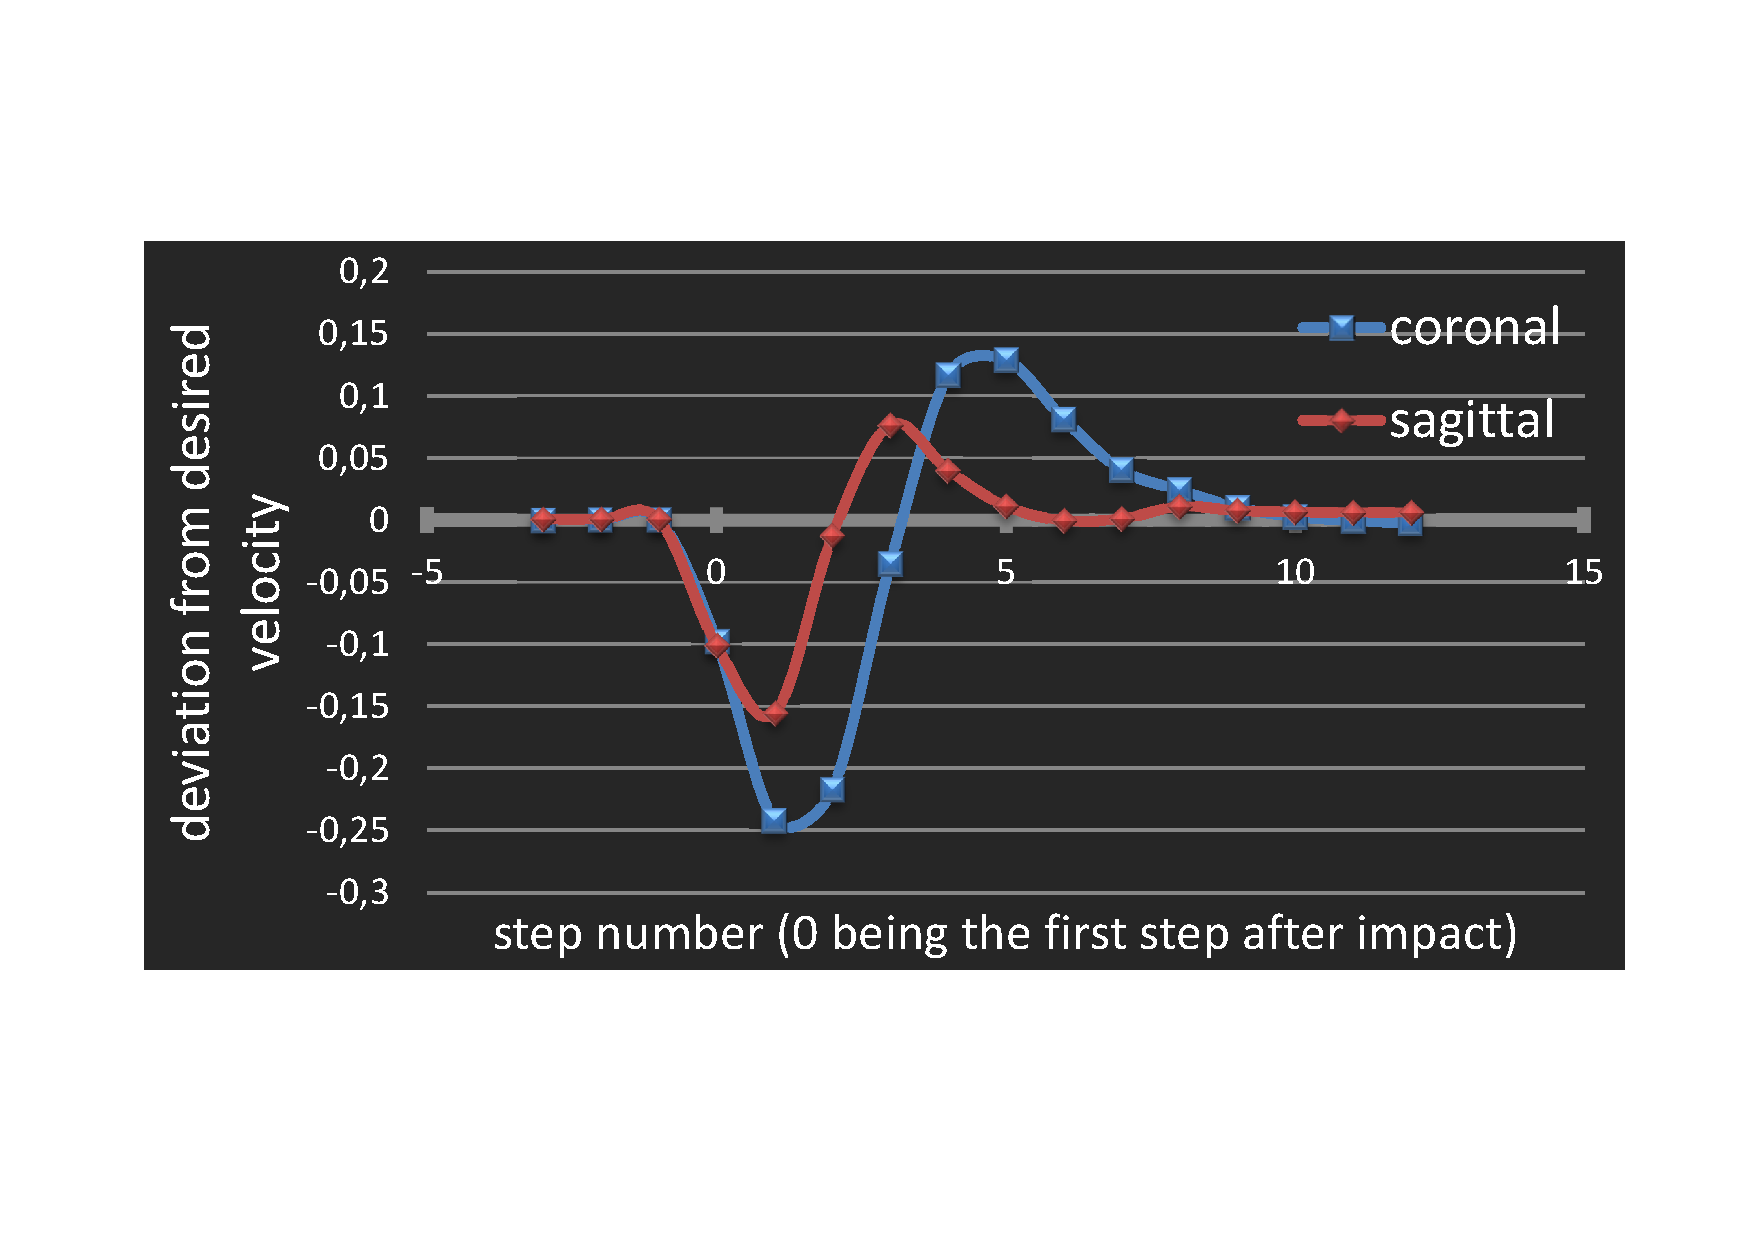
\includegraphics[scale=0.255]{images/strips/ball/speed_evo_after_impact.pdf}
\end{minipage}

\caption{Results obtained with our final controller. From top to bottom: character walking in 25cm, 50cm and 75cm of water. Right: character recovering from an external push, left: impact image, right: curves for the velocity deviation from the target velocity observed after impact. The character is moving at $0.6m.s^{-1}$ in all the presented situations with no coronal speed.}
\label{fig:controller_results}
\end{figure}

Our controller allows online modification of the character's target velocity. It is also possible to change the step width during movement. The controller is able to adapt to water height (figure~\ref{fig:controller_results}) as well as changes to the liquid's physics properties (density and viscosity). Our system is able to withstand external forces simulated through solid balls of 5kg projected onto the character (figure~\ref{fig:controller_results} bottom). All the simulations respect the real-time condition with a minimum of 27 fps when the water reaches the hips.

Figure~\ref{fig:controller_results} illustrates some of the results. The first two rows show that the character adapts the height of the swing foot to reach the water height. The third row illustrates the case where the water height is too high and the character keeps the swing foot near the ground. The right images illustrate the character's recovery after an impact from a $5kg$ ball moving at $5.4m.s^{-1}$. As we can see, numerous steps are necessary to return to a stable velocity.
The controller obtained by the presented optimization can precisely track any target sagittal speed from $0.2m.s^{-1}$ to $0.8m.s^{-1}$ under water height up to 1m and $1.0m.s^{-1}$ if the water height is lower than the knees. The following tests have been realized for a $0.6m.s^{-1}$ forward walk. The range of coronal speeds that can be achieved goes from $-0.25m.s^{-1}$ to $0.25m.s^{-1}$ under water height up to 1m. The controller can adapt to liquids with a density up to 1.5 times the density of water and. The character is robust to external pushes up to $5kg$ balls moving at $6m.s^{-1}$.
\subsection{Discussions}

In this work, we have focused on obtaining real-time simulations over having an extensive realism. Our controller could benefit from a more realistic water model that would still comply with the real-time constraint.
Our system still uses a static threshold to detect the need for recovery steps instead of using an adaptive value depending on if the velocity learning has been completed or not. Using experimental results should be a correct solution to identify how the threshold should be adapted.
Our system presents some difficulties to reach the target coronal velocities especially if the desired variation is sudden. This is most likely caused by the fact that we need two learning velocity curves for the coronal axis. Adding a learning system with complex impact of the evolution of one curve on the other could be a possible solution.

\section{Conclusion}
\label{sec:conclusion}

We have presented a physics-based controller capable of real-time interactive simulation of walking motions for partially immersed bipeds. We have demonstrated online adaptation of the gait style to external conditions such as the liquid height and target character's velocity. Our controller permits the specification of new gait styles specific to walking motions in a liquid medium.

This projet has been set up with the initialization of a research axis on motion control and will be continued during a Ph.D.. A paper has been submitted in july for the conference Motion In Games (MIG). I worked independently with the help of my supervisors during this project.

Our controller could be extended by implementing a more realistic liquid model which could consider the perturbations of the liquid caused by the character. Adding other mediums (e.g. snow-like mediums) or movement types (e.g. standing still, running…) with possible online transition between them are also interesting works we would like to investigate. Working on a non rigid model for the feet would improve the controller as well by bringing more advanced balance strategies and more realistic interactions between a virtual human and its environment. 
 
%\section*{Acknowledgements}

%\nocite{*}

\bibliography{template}
\end{document}
